% !TEX root = Master.tex

In this chapter, we explore diverse ways on how to model, evaluate and interpret the dependence structure of unit sales. 
%We first start at key category cluster level and compare the capabilities of the tried and tested methods on article unit sales. 
\\


%When we aggregate our data, not only promotion intensities need to be adapted. In the course of this, we average the total markdown percentage of all articles belonging to a respective aggregation group, e.g. each key category cluster obtains its own mean total markdown percentage. However, when we are trying to model dependence measures of pairwise groups as functions of covariates, we need a unifying feature for those groups. Luckily, we can readily average the aggregated total markdown percentages. \autoref{fig:total_markdown_pct_kcc} clarifies the strong linear correlations of those aggregated markdown percentages, therefore this simple solution should be rational. \\


%\begin{figure}[H]
%\centering
 % 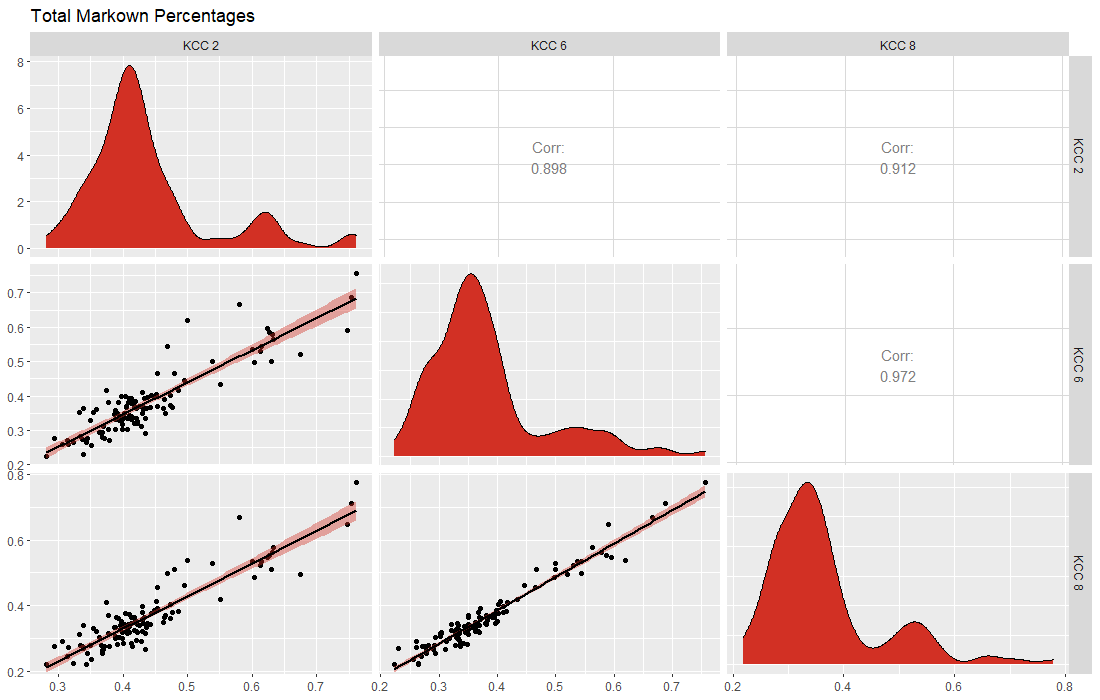
\includegraphics[width=0.8\linewidth]{figures/total_markdown_pct_kcc.png}
%  \caption{Pairwise total markdown percentages of key category clusters}
%  \label{fig:total_markdown_pct_kcc}
%\end{figure}

An important aspect of the modelling part is that usually, continuous responses are implied in the literature. Nevertheless, discrete responses (like in our "real" case) are also justified when explanatory variables are involved. A detailed explanation can be found in \cite{trivedi2017note}.\\ 
As the observation period is only 109 weeks and the highest peaks occur during Black Friday twice, the second time being very late (104th week, see e.g. \autoref{fig:total_sold_articles_ts}), all of the modelling is being performed in-sample. Thus, evaluation and diagnostics are based on the entire observation period so that both extreme peaks can be included in model trainings.\\
This chapter starts with Section \ref{ssec:kcc_margins}, where we fit the logarithmic sales (semi-)parametrically within the \ac{GAMLSS} framework. Next, in Section \ref{ssec:kcc_copulas}, we use a conditional copula approach using the residuals of Section \ref{ssec:kcc_margins} as responses in order to obtain correlation structures between the key category cluster pairs. In Section \ref{ssec:article_dependencies}, a short application of a dynamic Bayesian network is introduced. Section \ref{ssec:discussion} contains a summarizing discussion about the chapter as well as an outlook for potential future research.


